\section{Introduction}

This document defines the WISEBED Federation API version 2.1 -- the `WISEBED API'. This API is designed to support i) the {\em control} of an experiment, ii) the federation of testbeds for experiments, and iii) the interactions required between testbeds in support of {\em virtual links}.

The API has been designed to enable a strong separation between the {\em controller} of an experiment and the testbed(s) ({\em testbed service(s)}) being controlled, to the extent that the controller software can be either co-located with the testbed services, or located on the testbed user's personal computer. In support of this the API is divided vertically into two `roles'; the testbed service role, and the controller role. The testbed service role implements all of the functions which are directed at a testbed; while the controller role implements the functions which are directed at a controller (often these are responses to functions previously directed at a testbed by that controller). This division is shown in figure \ref{fig:api_concept}. %A controller typically acquires a reference to a testbed service role instance and informs that instance of a reference to itself.

\begin{figure}[htb]
\centering
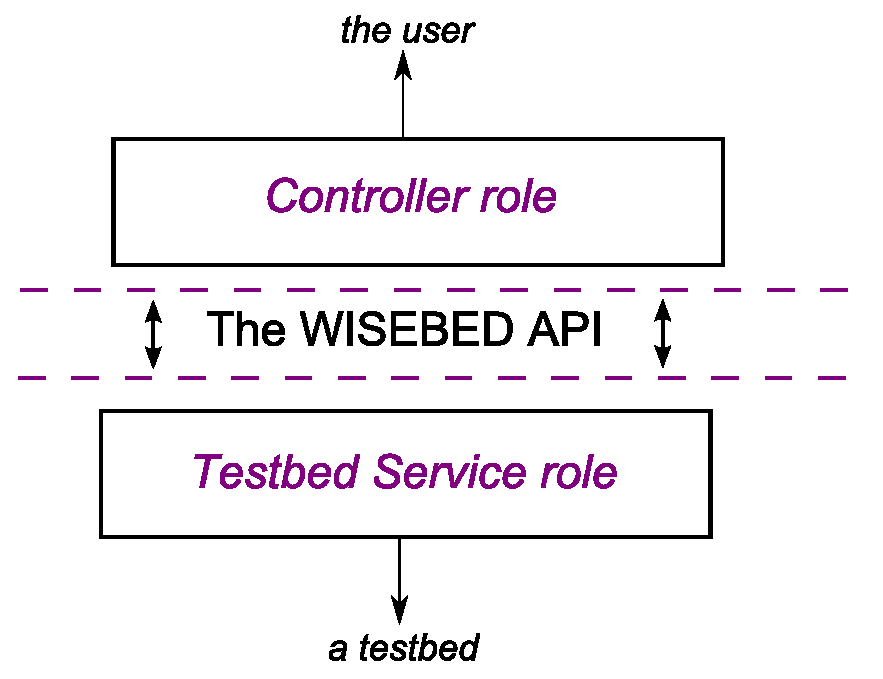
\includegraphics[height=160pt]{images/APIconcept}
\caption{Vertical division of API roles; each role has a set of functions from the API that it must implement}
\label{fig:api_concept}
\end{figure}

At the level of the testbed service role, the API is also divided into two parts horizontally: a {\em singleton} (always-available) part, and an {\em instantiable} part, a reference to which is provided by the singleton part in the form of a URN. This allows both decoupling of the location of a testbed service implementation, and an instance-per-experiment approach which removes the need to have any kind of `session key' parameter to every API call in order to distinguish different concurrent users of a testbed service\footnote{It does not however preclude the instantiable part also being a singleton in single-use testbeds; in this case the same instance reference would always be returned.}. This is illustrated in figure \ref{fig:api_concept2}.

\begin{figure}[htb]
\centering
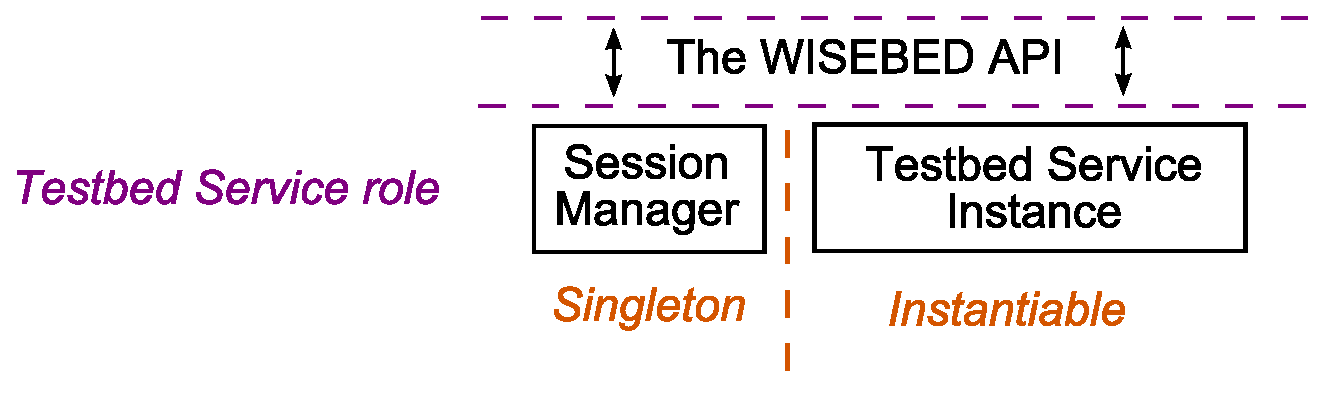
\includegraphics[height=80pt]{images/APIconcept2}
\caption{Horizontal division within the testbed service role; a testbed service instance reference is generated by a Session Manager}
\label{fig:api_concept2}
\end{figure}

Implementations of the WISEBED API are designed to be hierarchically composable, such that one instance can drive -- and receive feedback from -- another instance. This also means that an entity controlling an experiment -- driving a WISEBED API -- does not need to be aware of a possible hierarchy of API instances below that `root' instance, permitting arbitrary federations and virualisations of testbeds that are controllable by the same controller. Furthermore a controller generally needs little or no knowledge of any `session' identifier due to the API instancing capability. Example compositions are shown in figure \ref{fig:api_concept3} ({\bf TODO: Show a TARWIS-esque setup purely using web-based access of a single testbed, and other versions \ref{todo}}).


\begin{figure}[htb]
\centering
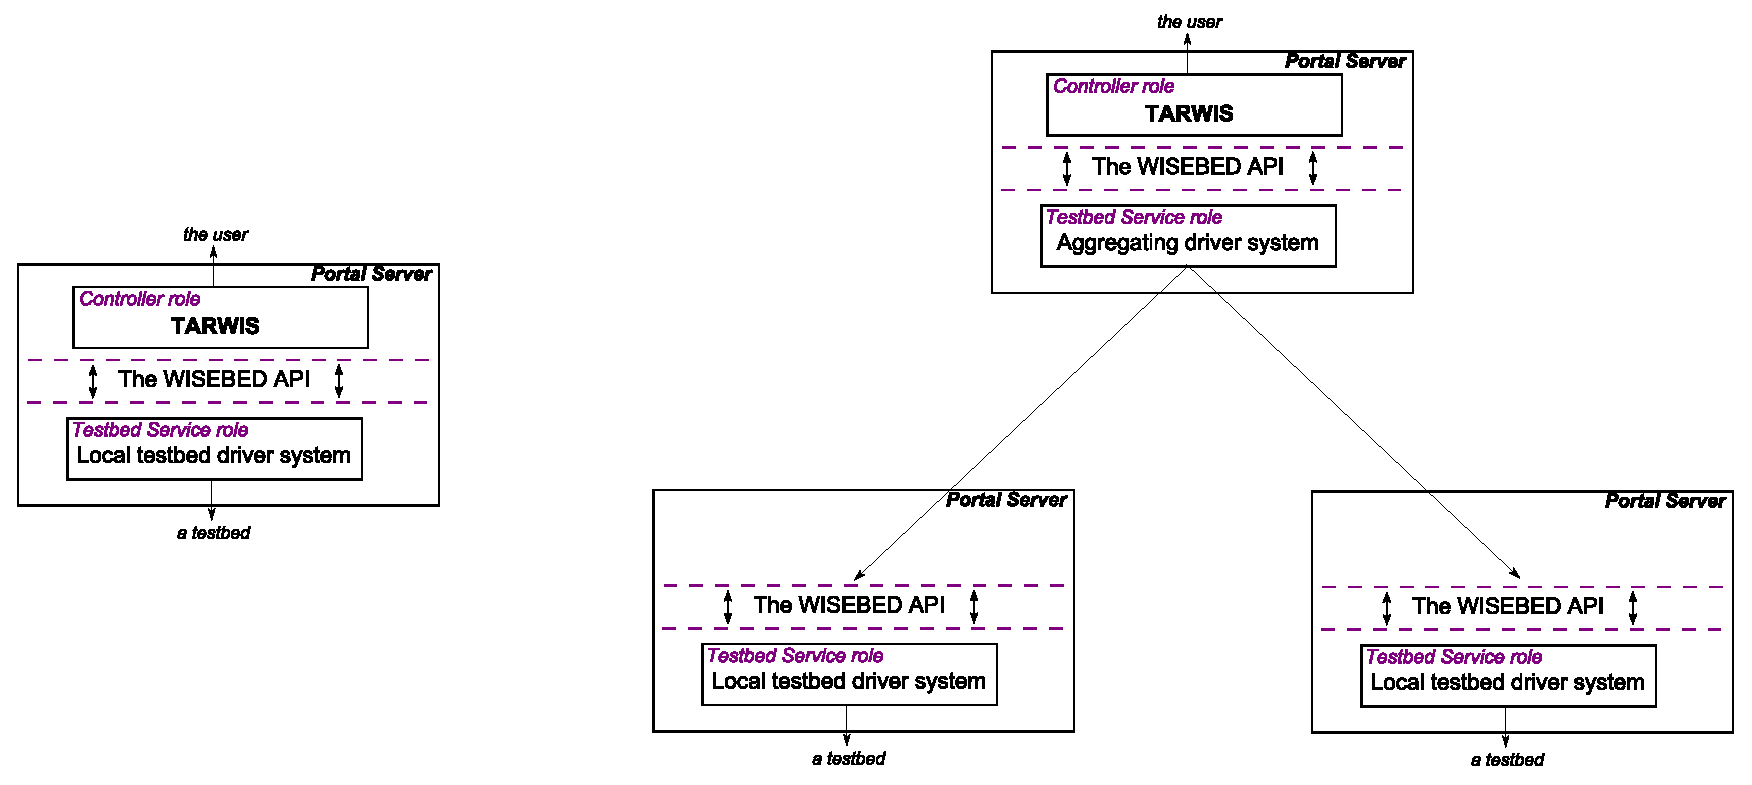
\includegraphics[height=150pt]{images/APIconcept3}
\caption{Horizontal division within the testbed service role; a testbed service instance reference is generated by a Session Manager}
\label{fig:api_concept3}
\end{figure}


The general flow of control for a user of the WISEBED federation is therefore as follows: They are first authorized to use the federation and authenticated by an external security system (e.g. via some web-based sign-up procedure). They then use an external reservation system (again perhaps through a website) which provides that user with access to selected testbed resources at some point in the future and returns to them a `reservation ID'. The details of both of these systems are beyond the scope of this document. When a user's reserved time arrives they -- or a system working on their behalf -- can use their reservation ID to acquire the reference(s) to the testbed service instance(s) at the revelant site(s). These instances will be destroyed automatically when their reserved time expires. %this last part is new


This version of the WISEBED API is as agreed during discussions about virtual link support (hosted at UZL, 2nd-4th September 2009) between partners RACTI, TUBS, ULANC and UZL, and follows from the previously discussion WSN API 2.0.
